\documentclass{article}
\usepackage{amssymb}
\usepackage[utf8]{inputenc}
\usepackage{geometry}
\usepackage{mathtools}
\usepackage{verbatim}

\geometry{letterpaper, portrait, margin=1in}

\title{CS325 - Project 2}
\author{Group \#6 \\ William Jernigan, Alexander Merrill, Sean Rettig}
\date{\today}

\begin{document}

\maketitle

\section*{Correctness}
\subsection*{Proof of Claim 3: Direct Proof}

\begin{quote}
Claim 3: If $\{z_{1},z_{2},...,z_{t}\}$ and $\{z_{1},z_{2},...,z_{s}^{'}\}$ are two visible sets of lines (each ordered by increasing slope), then the visible subset of $\{z_{1},z_{2},...,z_{t}\}\cup\{z_{1},z_{2},...,z_{s}^{'}\}$ is $\{z_{1},...,z_{i}\}$ for some $i \leq 1$ and $j \leq s$.
\end{quote}

\subsubsection*{Prove that $\{a_{1},...,a_{i}\}$ is visible}
    Because all elements in A were defined to be visible with respect to each other, any covering line $b_{q}$ must be from B.\\
    Given that $m_{a_{t}} < m_{b_{1}}$, a covered line $a_{p} \in A$ has $m_{p} < m_{q}$.
    
    \paragraph{Prove that for any covered line  $a_{p}, p = i + 1$, all lines to the right of p in A are also covered:}
        Because $a_p$ is defined to be invisible, then by Claim 2 in the P1 Visible Lines Handout:\\
        $y_{a_{p-1}}(x_{a_{p-1}, b_{q}}) > y_{a_{p}}(x_{a_{p-1},b_{q}})$, where $x_{a_{p-1}, b_{q}}$ is the x coordinate where $a_{p-1}$ and $b_q$ intersect.\\
        Because $a_{p+1}$ is defined to not cover $a_p$, we know that $y_{a_{p}}(x_{a_{p-1}, b_{q}}) > y_{a_{p+1}}(x_{a_{p-1},b_{q}})$.\\
        For $x < x_{a_{p-1},a_{p}}, a_{p+1}$ is covered by $a_p$.\\
        We need to show that $a_{p+1}$ is covered for $x \geq x_{a_{p-1},a_{p}}$.\\
        Because $b_q$ is covering $a_p$, $y_{b_{q}}(x) > y_{a_{q}}(x)$ for $x \geq x_{a_{p-1},b_{q}} \geq x_{a_{p-1},a_{p}}$.\\
        \therefore $p+1$ is invisible if p is invisible.\\
        This follows for all p.
Then let $p = i + 1$. \therefore $\{a_1,...,a_i\}$ is visible and $\{a_p,...,a_t\}$ is invisible.\\
Do the same thing for set B.


\subsection*{Proof of Algorithm 4: Inductive Proof}
    Let $Y$ be a list of $n$ lines sorted in ascending order by slope. We claim that Algorithm 4 can determine which lines are visible in the set.
    \subsubsection*{Base case:} If $n \leq 2$, the lines are trivially visible because no line two lines exist to cover any single line.
    \subsubsection*{Inductive hypothesis:} For $n \geq 3$, Algorithm 4 can split $Y$ in half, determine visibility for each half, and then merge them.
    \subsubsection*{Applying the axiom of induction:} Let $A$ be the first half of $Y$ and $B$ be the second half of $Y$. Let all lines in $A$ be visible w.r.t. one another. Let all lines in $B$ be visible w.r.t. one another. Let $V$ be the set of visible lines in $Y$, which trivially includes the first line in $A$ and the last line in $B$ since no line exists with lesser slope or greater slope, respectively. Next, take $i$ to be an index of a line in $A$, starting at the second line (if length of A is 1, disregard). Also, take $j$ to be an index of a line in $B$, starting at the second to last line (if length of B is 1, disregard). 
    We can check if lines $A_{i}$ and $B_{j}$ are visible by testing them with Claim 1 and the lines most recently added to $Y$ from $A$ and $B$. If $A_{i}$ (or $B_{j}$) is visible, we will add $A_{i}$ (or $B_{j}$) to $V$, increase $i$ (or decrease $j$), and check the new $A_{i}$ (or $B_{j}$) the same way. If the index cannot be incremented, you are done. If $A_{i}$ (or $B_{j}$) is not visible, we know by Claim 3 that the rest of the lines to the right of $A_{i}$ (or to the left of $B_{j}$) are not visible, so we will stop checking for visible lines in $A$ (or $B$).


\section*{Experimental and Asymptotic Run Time Analysis}
\subsection*{Experimental Run Time Data}
\verbatiminput{times.txt}

\pagebreak

\subsection*{Experimental Run Time Plots}
\centerline{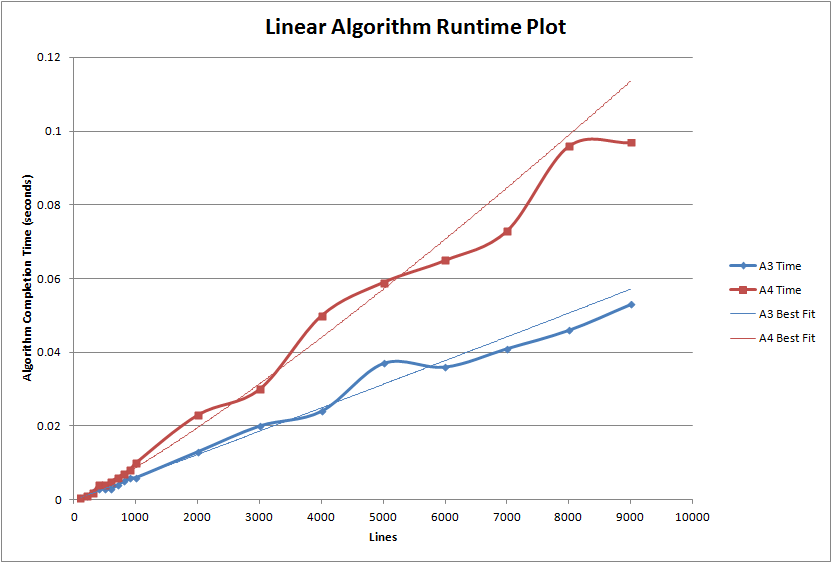
\includegraphics[width=0.75\textwidth]{plot1.png}}
\centerline{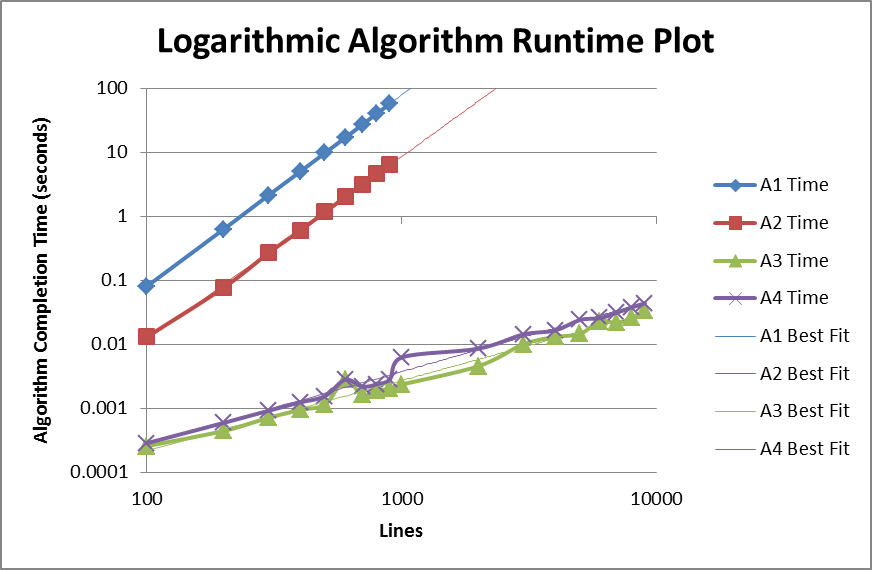
\includegraphics[width=0.75\textwidth]{plot2.png}}

\pagebreak

\subsection*{Experimental Run Time Analysis}
Algorithm 3: $y=5 \times 10^{-6}x^{1.0234}$\\
Algorithm 4: $y=3 \times 10^{-6}x^{1.1695}$\\

Given these equations, we can use both the slopes and our code to analyze the run times of the algorithms. We can also determine the biggest instance that can be solved with each algorithm in an hour.

\subsection*{Asymptotic Run Time Analysis}
Algorithm 1: $\Theta(n^3)$\\
Algorithm 2: $\bigcirc(n^3)$\\
Algorithm 3: $\bigcirc(n^2),\Omega(n)$\\
Algorithm 4: $\bigcirc(nlogn),\Omega(logn)$\\
\indent Algorithm 4 

\subsection*{Extrapolation and Interpretation}
\subsubsection*{Estimated Number of Lines Per Hour}
Algorithm 3: $y=5 \times 10^{-6}x^{1.0234}$\\
Algorithm 4: $y=3 \times 10^{-6}x^{1.1695}$

\subsubsection*{Discrepancies}
%The theoretical run-time for Algorithm 4 is theoretically faster than that of Algorithm 3 however the experimental run-time is slower. This is likely due to how Python and the processor handle our code. Since both have linear run-times, it's likely that the constants for Algorithm 4 are largely, which could be due to how our code is handled by the Python compiler or how it's processed. For example, this could be due to Algorithm 4 creating more arrays than Algorithm 3 and creating and tearing down arrays being more time intensive.

We note that the slopes from our experimentally-derived equations are within the asymptotic run-time range of $\bigcirc(n^2)$, $\Omega(n)$ and $\bigcirc(nlogn)$, $\Omega(logn)$ however Algorithm 4, which is theoretically faster than Algorithm 3 actually runs slower. This discrepancy many have many possible contributing factors, including a small sample size, a low timing resolution (particularly for Algorithm 3), how the compiler and system handle arrays and operations, and randomness in run-time present. This randomness in run-time is due to both Algorithms not performing a fixed number of operations, but rather change what operations they run depending on the input lines given. The randomness and how the compiler and system handle the our code are likely the primary causes of these differences.

\pagebreak

\section*{Pseudocode}
\verbatiminput{pseudocode.txt}

\end{document}
